\section{Information Theory and Dimensionality Reduction}
The following section provides a short introduction into information theory and optimal coding.
For a more comprehensive introduction it is recommended to look into 
\cite[Chapter 6 \& 7]{Applebaum2008}. In the previous section we have talked about
model comparison and we will follow this conception from an information theoretic
point of view.
We have earlier used the likelihood as a measure for model comparison and we will use it now
to introduce an information theoretic measure, the cross-entropy. Strictly speaking, the
likelihood function maps a set of possible models to a real value, given an observed data
set. We recognize that the likelihood function is not a probability density function, as it is
not normalized.

\begin{proposition}[Cross-entropy]
Given: We have observed a set of data point $D$ generated from a random variable $X \sim \rho(x)$, with
$\rho(x)$ being unknown to us, and we want to represent the data using the model $\hat{\rho}(x)$. 
The probability of i.i.d. samples $\{x_1, x_2, x_2, \dots x_N\}$
under the model $\hat{\rho}(x)$ is given by
\begin{align*}
	p(D|\hat{\rho}) = \prod_{n=1}^N \hat{\rho}(x_n)
\end{align*}
and 
\begin{align*}
	\log L(D;\hat{\rho}) = \log p(D|\hat{\rho}) = \sum_{n=1}^N \log \hat{\rho}(x_n)
\end{align*}
is the log-likelihood. We find the empirical expectation of a function by using the normalized
sum over all observations, such that for the expected log-likelihood we find
\begin{align}
	\begin{split}
	   \Exest{}{\log \hat{\rho}(x)} &= \frac{1}{N} \sum_{n=1}^N \log \hat{\rho}(x_n) \\
	   							     &= \Ex{\rho_{emp}(x)}{\log \hat{\rho}(x)}
	\end{split}
\end{align}
where
\begin{align*}
	\rho_{emp}(x) = \frac{1}{N} \sum_n \delta(x - x_n)
\end{align*}
is the empirical distribution of $x$. That is, the empirical expectation of the log-likelihood
is an expectation with respect to the empirical distribution $\rho_{emp}(x)$. We notice that 
if the number of observations approaches infinity the empirical distribution is equal to
$\rho(x)$:
\begin{align*}
	\lim_{N \rightarrow \infty} \rho_{emp}(x) = \rho(x)
\end{align*}
Following this observation the expected negative log-likelihood for infinitely many observations
can be written as:
\begin{align*}
	\lim_{N \rightarrow \infty} \left( \Ex{\rho_{emp}(x)}{- \log \hat{\rho}(x)} \right)
				&= \Ex{\rho(x)}{- \log \hat{\rho}(x)} 
\end{align*}
where 
\begin{align}
	\Ex{\rho(x)}{- \log \hat{\rho}(x)} \stackrel{\text{cont.}}{:=} - \int_{X}\rho(x) \log \hat{\rho}(x) \, \mathrm{d}x
\end{align}
is called the cross-entropy of using probability distribution $\hat{\rho}(x)$ to represent data
from the true distribution $\rho(x)$. For the \emph{discrete case} the cross-entropy is given by
\begin{align}
	\Ex{p(x)}{- \log p(x)}
		&\stackrel{\text{disc.}}{:=} - \sum_{x \epsilon X} p(x) \log \hat{p}(x)
\end{align}
In information theory the cross-entropy is a measure of the expected code length needed to respresent
events from the probability distribution $\rho(x)$ using another probability distribution
$\hat{\rho}(x)$. We will later see how to understand this definition.
\end{proposition}

%The cross-entropy
%is a measure of the expected information needed to identify an event $A$ from the 
%sample space $S$ given we code random variable $X$  by $\hat{\rho}(x)$ rather than $\rho(x)$.
%For the \emph{continuous case} we define the cross-entropy as
%	\begin{align}
%		\mathrm{E}_{\rho(x)}\left[-\log \rho (x) \right] 
%			&\stackrel{\text{cont.}}{:=} - \int_{X}\rho(x) \log \hat{\rho}(x) \, \mathrm{d}x
%	\end{align}
%where
%	\begin{align}
%		\mathrm{I}(A) = -log_b\rho(A)
%	\end{align}
%is called the information content of an event $A$. Due to the monotonicity of the logarithm,
%we see that $\mathrm{I}(A) \rightarrow 0$ for $\rho(A) \rightarrow 1$. That is, information can be seen
%as a measure of 'surprise'. If an event if very likely it's information content is low, whereas
%if an event is very unlikely it's information content is  high.
%It should be noted that the logarithm is taken to the
%base $b$ dependent on the coding scheme which defines the unit of information. $b = 2$ for example 
%corresponds to a coding scheme in \emph{bits} and $b = \mathrm{e}$ corresponds to a coding scheme
%in \emph{nats}. Similar to the continuous case we can measure the cross-entropy for the
%\emph{discrete case} using
%	\begin{align}
%	 		\mathrm{E}_{p(x)}\left[-\log p (x) \right]
%			&\stackrel{\text{disc.}}{:=} - \sum_{x \epsilon X} p(x) \log \hat{p}(x)
% 	\end{align}
%In general the cross-entropy is a measure of the expected code length needed to respresent
%events from the probability distribution $\rho(x)$ using another probability distribution
%$\hat{\rho}(x)$.
%\end{proposition}
%
%Training set for different classes
%
%$c = 0, \dots, 9 $
%
%$\hat{\rho}(\hat{x} | c) = 
%      \mathcal{N}(\underbrace{\mathbf{U}_c\TT \mathbf{x}}_{\mathbf{s}} | 
%                  \boldsymbol \mu_c, \sigma_{1c}^2	, \dots, \sigma_{dc}^2)$
%                  
%The log-likelihood of the data is equal to tha negative cross-entropy of the model given the data.
%
%Test sets:
%$\rho(\mathbf{x} | c^*) =\frac{1}{N} \sum_{\mathbf{x_k} \, \epsilon \, \text{testset}} \delta(\mathbf{x} - \mathbf{x_k})$
%
%$ \Rightarrow \text{cross-entropy} \hat{=} 
%    - \sum_{\mathbf{x_k} \, \epsilon \, \text{testset*}} \log \hat{\rho} (\mathbf{x_k}|c)$
%    
%$\mathrm{E}_{\rho_{emp}} \left[ f(\mathbf{x}) \right] = \frac{1}{N} \sum_{k = 1}^N f(\mathbf{x_k}) $
%
%exp(neg cross-entropy) $:=$ likelihood of the model for the entire test set

\subsection{Consider the best model}
We have learned earlier that the true model $\rho(x)$ has largest likelihood 
given the data is generated from $\rho(x)$. That is, if the expected log-likelihood is maximized
then the expectation of the negative log-likelihood will be minimal such that
\begin{align}
   &\lim_{N \rightarrow \infty} \left( \frac{1}{N} \sum_{k = 1}^N -\log \rho(\mathbf{x_k}) \right)
   = - \int \rho (\mathbf{x}) \log \rho(\mathbf{x}) \mathrm{d}\mathbf{x} 
\end{align}   
is minimal for the true generating model $\rho(x)$. We call 
\begin{align}
	  \mathrm{h}[X] &\stackrel{\text{cont.}}{:=} - \int \rho (\mathbf{x}) \log \rho(\mathbf{x}) \mathrm{d}\mathbf{x}
\end{align}
the \emph{differential entropy} of a continuous random variable X with 
$\mathrm{h}[X] \, \epsilon \, \mathbb{R}$. An eqivalent definition for the case of discrete 
random variables has the form
\begin{align}
	\mathrm{H}[x] = - \sum_{k=1}^K p(x_k) \log p(x_k)
\end{align}
with $\mathrm{H}[x] \, \epsilon \, \mathbb{R}^+$. This is called the \emph{discrete entropy}.
The entropy measures the minimal discription length, or the most compact description, of a random
variable. The description length of a random variable will be minimal if the code which describes
the random variable comes from true distribution of that random variable. The negative log-probability
of an observation approximates the code word length for describing that observation.

\subsection{Information}
In information theory the negative log probabilty of an event $A$ under a model $\rho(x)$
	\begin{align}
		\mathrm{I}(A) = -log_b\rho(A)
	\end{align}
is called the information content of an event $A$. Due to the monotonicity of the logarithm,
we see that $\mathrm{I}(A) \rightarrow 0$ for $\rho(A) \rightarrow 1$. That is, information can be seen
as a measure of 'surprise'. If an event if very likely it's information content is low, whereas
if an event is very unlikely it's information content is  high.
It should be noted that the logarithm is taken to the
base $b$ dependent on the number of symbols in the alphabet which defines the unit of information. 
$b = 2$ for example corresponds to a binary code which is represented in \emph{bits}, whereas
$b = \mathrm{e}$ corresponds to a coding scheme in \emph{nats}.

\begin{exbox}{Discrete distribution (uniform)}
Given a discrete random variable $X$ such that
\begin{align*}
	x \, \epsilon \, \{1,2,3,4\} \qquad p(x) = \frac{1}{4}
\end{align*}
Then for a binary code the entropy is given by:
\begin{flalign*}
	\mathrm{H}[p(x)] &= - \sum_{x = 1,2,3,4} p(x) \log p(x) \\
	 				 &= - \log_2 \frac{1}{4} \\
	 				 &= \log_2 4 = 2 [bits]
\end{flalign*}
Whereas for a terniary code with three symbols the entropy is given by:
\begin{flalign*}
\mathrm{H}[p(x)] &= - \sum_{x = 1,2,3,4} p(x) \log p(x) \\
	 				 &= - \log_3 \frac{1}{4} \\
	 				 &= \log_3 4 \approx 1.26 [trits]
\end{flalign*}

Binary alphabet: $p(x) = \frac{1}{8} \Rightarrow \mathrm{H}[p(x)] = 3\mathrm{bits}.$ \\
Ternary alphabet: $p(x) = \frac{1}{9} \Rightarrow \mathrm{H}[p(x)] = 2\mathrm{trits}.$ \\

\end{exbox}


\subsubsection{Optimality}
We understand optimality in the sense that for \emph{infinitely long} sequences of observations 
the description length takes a minimum and that this minimum description length is tightly bounded
by the entropy such that:
\begin{align}
	\mathrm{H}[x] \leq \frac{\# \text{symbols}}{\# \text{words}} \leq \mathrm{H}[x] + 1
\end{align}
where $\frac{\# \text{symbols}}{\# \text{words}}$ is the the average code word length. This
is called "Shannon's noiseless coding theorem".

\subsection{Quantization}
Problem: The description length of a continuous random variable is infinite. However, we can introduce a quantization which divides the variable space into equally sized bins of size $\Delta$. By this we are mapping a continuous RV into a discrete space such that we can calculate the discrete Entropy $\mathrm{H}_\Delta$ under the quantization $\Delta$.

\begin{wrapfigure}{r}{0.5\textwidth}
	\centering
	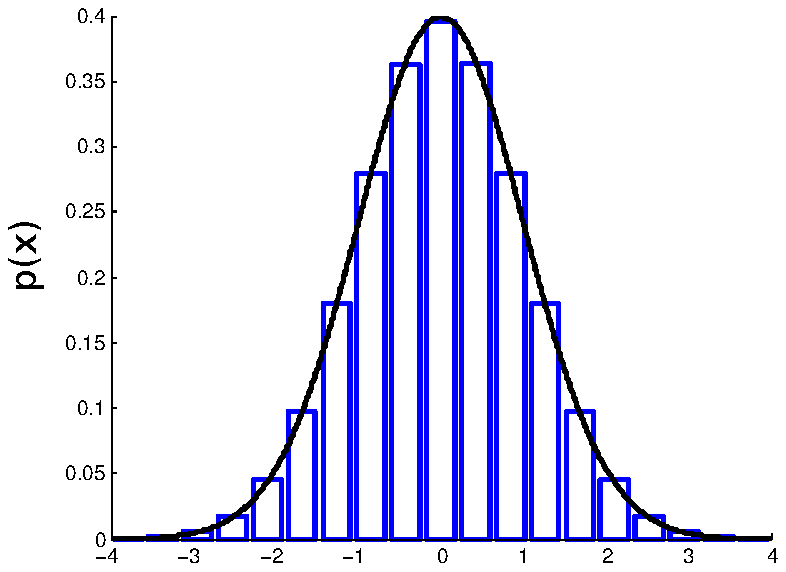
\includegraphics[width=0.45\textwidth]{./lecture12/gauss_quant.pdf}
	\caption{Quantization of a normally distributed random variable.}
\end{wrapfigure}
The 
\begin{align}
	{H}_\Delta[x] \approx \mathrm{h}[x] - \log \Delta
\end{align}

It can be shown that:
\begin{align}
	\mathrm{h}[x] = \lim_{\Delta \rightarrow 0} \left( \mathrm{H}_\Delta[x] + \log \Delta \right)
\end{align}

Maximum likelihood classification follows the minimum description length principle, 
i.e. find the model that corresponds to the most compact description of the data.

\subsection{Joint entropy}
\begin{definition}[Joint entropy]
Discrete case:
\begin{align*}
		\mathrm{H}[X,Y] = -\sum_{x_k,y_j} p(x_k,y_j) \log p(x_k,y_j)
\end{align*}

Continuous case:
\begin{align*}
		\mathrm{h}[X,Y] = - \mathop{\int \! \! \! \int} \rho(x,y) \log \rho(x,y) \, \mathrm{d}x \mathrm{d}y
\end{align*}
\end{definition}

\subsection{Mutual Information}

\begin{align*}
	\underbrace{\mathbf{X}}_{\text{Source}} \stackrel{\text{channel}}{\longrightarrow} \underbrace{\mathbf{Y}}_{\text{Receiver}}
\end{align*}


\begin{example}[Channel coding with shared bits]
	Given: A bit code with 8 possible words
	\begin{align*}
		\mb{b} \, \epsilon \, \{0,1\}^3 = \{000,001,010,011,100,101,110,111\}
	\end{align*}
	and equal probabilities of word occurences
	\begin{align*}
		\qquad p(\mathbf{b}) = \frac{1}{8}
	\end{align*}	  
	Source and Receiver share one bit such that
	\begin{align*}
 		\mb{x} = \begin{pmatrix} b_1 \\ b_2 \end{pmatrix}; \qquad 
		\mb{y} = \begin{pmatrix} b_2 \\ b_3 \end{pmatrix}
	\end{align*} 	
	The optimal code word length for source and receiver is given by
	\begin{align*}
		\mathrm{H}[X] = 2 \, \mathrm{bits}; \qquad \mathrm{H}[Y] = 2 \, \mathrm{bits}
	\end{align*}
	and for the shared code
	\begin{align*}
			\mathrm{H}[X,Y] = 3 \, \mathrm{bits}
	\end{align*}
	We see that $\mathrm{H}[X,Y] \leq \mathrm{H}[X] + \mathrm{H}[Y]$ and that
	\begin{align*}
		\mathrm{I}[X:Y] = \mathrm{H}[X] + \mathrm{H}[Y] - \mathrm{H}[X,Y] = 1 \, \mathrm{bits}
	\end{align*}
	is the number of shared bits between source $X$ and receiver $Y$. This is called the mutual
	information of $X$ and $Y$.
\end{example}


\begin{definition}[Mutual information]
\begin{align*}
		\mathrm{I}[X:Y]
		      & \stackrel{\text{cont.}}{:=} \mathrm{h}[X] + \mathrm{h}[Y] - \mathrm{h}[X,Y] \\
   		      & \stackrel{\text{disc.}}{:=} \mathrm{H}[X] + \mathrm{H}[Y] - \mathrm{H}[X,Y]
\end{align*}
\end{definition}

\begin{figure}
	\centering
	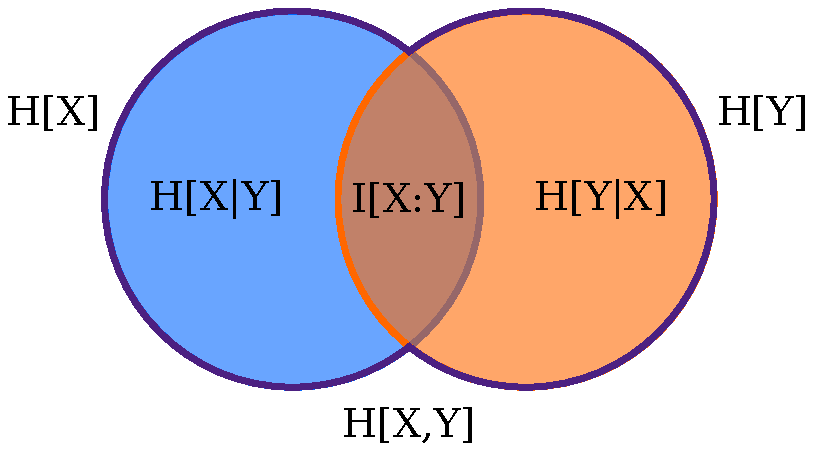
\includegraphics[width=0.45\textwidth]{./lecture12/venn.pdf}
	\caption{A Venn diagram for the relationship of information theoretic measures.}
\end{figure}

\subsubsection*{Reexpressing mutual information}
\begin{align}
\begin{split}
	\mathrm{I}[X:Y] &= \mathrm{h}[X] + \mathrm{h}[Y] - \mathrm{h}[X,Y] \\
	                &= - \int \rho (\mathbf{x}) \log \rho(\mathbf{x}) \mathrm{d}\mathbf{x} 
	                   - \int \rho (\mathbf{y}) \log \rho(\mathbf{y}) \mathrm{d}\mathbf{y} 
	                   + \mathop{\int \! \! \! \int} \rho(x,y) \log \rho(x,y) \, \mathrm{d}x \mathrm{d}y \\
	                &= \mathop{\int \! \! \! \int} \rho(x,y) \log \frac{\rho(x,y)}{\rho(x)\rho(y)} \, \mathrm{d}x \mathrm{d}y \\
	                &= \mathop{\int \! \! \! \int} \rho(x,y) \log \frac{\rho(x|y)}{\rho(x)} \, \mathrm{d}x \mathrm{d}y \\
	                &= \mathop{\int \! \! \! \int} \rho(x,y) \log \frac{\rho(y|x)}{\rho(y)} \, \mathrm{d}x \mathrm{d}y \\
	                &= \mathrm{h}[X] + \mathop{\int \! \! \! \int} \rho(x|y) \rho(y) \log \rho(x|y) \, \mathrm{d}x \mathrm{d}y \\
	                &= \mathrm{h}[X] - \underbrace{\int \rho(y) 
	                     \left(- \int \rho(x|y) \log \rho(x|y) \, \mathrm{d}x \right) \mathrm{d}y}_{\text{conditional entropy}} \\
	                &= \mathrm{h}[X] - \mathrm{h}[X|Y] \\
	                &= \mathrm{h}[Y] - \mathrm{h}[Y|X]
\end{split}
\end{align}
The conditional entropy $\mathrm{h}[Y|X]$ is the entropy of a random variable $Y$ conditioned on 
any possible outcome of random variable $X$. It corresponds to the number of additional bits
needed on average to code for $Y$ given that $X$ has been observed. It is a reflection of the uncertainty that
is introduced by the channel.

\begin{exbox}{Differential entropy of a Gaussian random variable}
	\begin{align*}
	\mathrm{h}[X] &= \frac{1}{2} \log_\mathrm{e} \left( 2 \pi \mathrm{e} \mathrm{Var}[X] \right) \text{in nats} \\
				  &= \frac{1}{2} \log_2 \left( 2 \pi \mathrm{e} \mathrm{Var}[X] \right) \text{in bits}
	\end{align*}
\end{exbox}